% Provenance (never printed): the firms strand of ../economics_series.md (grade 7: revenue, costs, profit, break-even,
% risk, entry and exit). Brief: sources/book1/BRIEFS.md, g7-08. Chart data: figdata/grade-7/08-firms (Eurostat business
% demography bd_size, enterprises born in 2021; Brenland firm census; the chapter's bakery example).
\chapter{Firms: Costs, Revenue and Profit}\label{ch:g7:firms}

\begin{openingchart}{Of 100 firms born in 2021, how many were still active one, two and
three years later: European Union and four of its countries.}{Eurostat, business
demography (bd\_size), survival rate of enterprises newly born in 2021, business economy}
\begin{tikzpicture}
\begin{axis}[omrecord, xmin=0, xmax=3, ymin=0, ymax=100, xtick={0,1,2,3},
  xlabel={Years after the firm was born}, ylabel={Firms still active (of 100)},
  legend style={at={(0.5,-0.2)}, anchor=north, legend columns=5}]
\pgfplotsforeachungrouped \col in {eu, nl, it, de, fr} {
  \addplot+[mark=*, mark size=1.5pt] table[x=years, y=\col] {figdata/grade-7/08-firms/out/survival.csv};
}
\legend{European Union, Netherlands, Italy, Germany, France}
\end{axis}
\end{tikzpicture}
\end{openingchart}

% figdata: facts (eu_y1 81.2, eu_y3 57.2, nl_y3 78.1, fr_y3 48.9, fi2019_y5 53.1, eu_births_2021_millions 3.4,
% eu_firms_2021_millions 31.5)
In 2021, about $3.4$ million new \omterm{def:g7:firms:firm}{firms} were born in the European Union, which had about
$31.5$ million \omterm{def:g7:firms:firm}{firms} in all. Of every 100 \omterm{def:g7:firms:firm}{firms} born that year, $81.2$ were still active a year later, and $57.2$ after three
years: more than four in ten had closed. The share differs between countries: $78.1$ of
100 were still active after three years in the Netherlands, $48.9$ in France. In Finland,
of 100 \omterm{def:g7:firms:firm}{firms} born in 2019, $53.1$ were still active five years later.

Why do people open \omterm{def:g7:firms:firm}{firms} when so many close? What decides whether a \omterm{def:g7:firms:firm}{firm} makes \omterm{def:g7:money:money}{money} or
loses it? This chapter follows the \omterm{def:g7:money:money}{money} of a \omterm{def:g7:firms:firm}{firm}: what it sells, what it pays, and what
is left.

\begin{recall}
A \omterm{def:g7:markets-and-prices:market}{market} is any arrangement where buyers and sellers meet and agree on exchanges
(\cref{ch:g7:markets-and-prices}). The \omterm{def:g7:scarcity-and-opportunity-cost:opportunity-cost}{opportunity cost} of a choice is the value of the best
option given up (\cref{ch:g7:scarcity-and-opportunity-cost}).
\end{recall}

\section{What a firm does}

\begin{definition}[Firm]\label{def:g7:firms:firm}
A \emph{firm}\index{firm} is an organisation that buys \omterm{def:g7:firms:input}{inputs} and uses them to produce goods
or services that it sells.
\end{definition}

\begin{definition}[Input]\label{def:g7:firms:input}
An \emph{input}\index{input} is anything a \omterm{def:g7:firms:firm}{firm} uses to produce: the work of its people,
materials, energy, machines, buildings, land.
\end{definition}

A bakery buys flour, yeast, energy and the work of its bakers, rents a shop and an oven, and
sells bread: its output. \omterm{def:g7:firms:firm}{Firms} range from one person selling at a \omterm{def:g7:markets-and-prices:market}{market} to companies with
hundreds of thousands of workers. Most \omterm{def:g7:firms:firm}{firms} are small.

\begin{definition}[Entrepreneur]\label{def:g7:firms:entrepreneur}
An \emph{entrepreneur}\index{entrepreneur} is a person who starts or runs a \omterm{def:g7:firms:firm}{firm} and bears the
risk of its losses.
\end{definition}

\begin{omfigure}
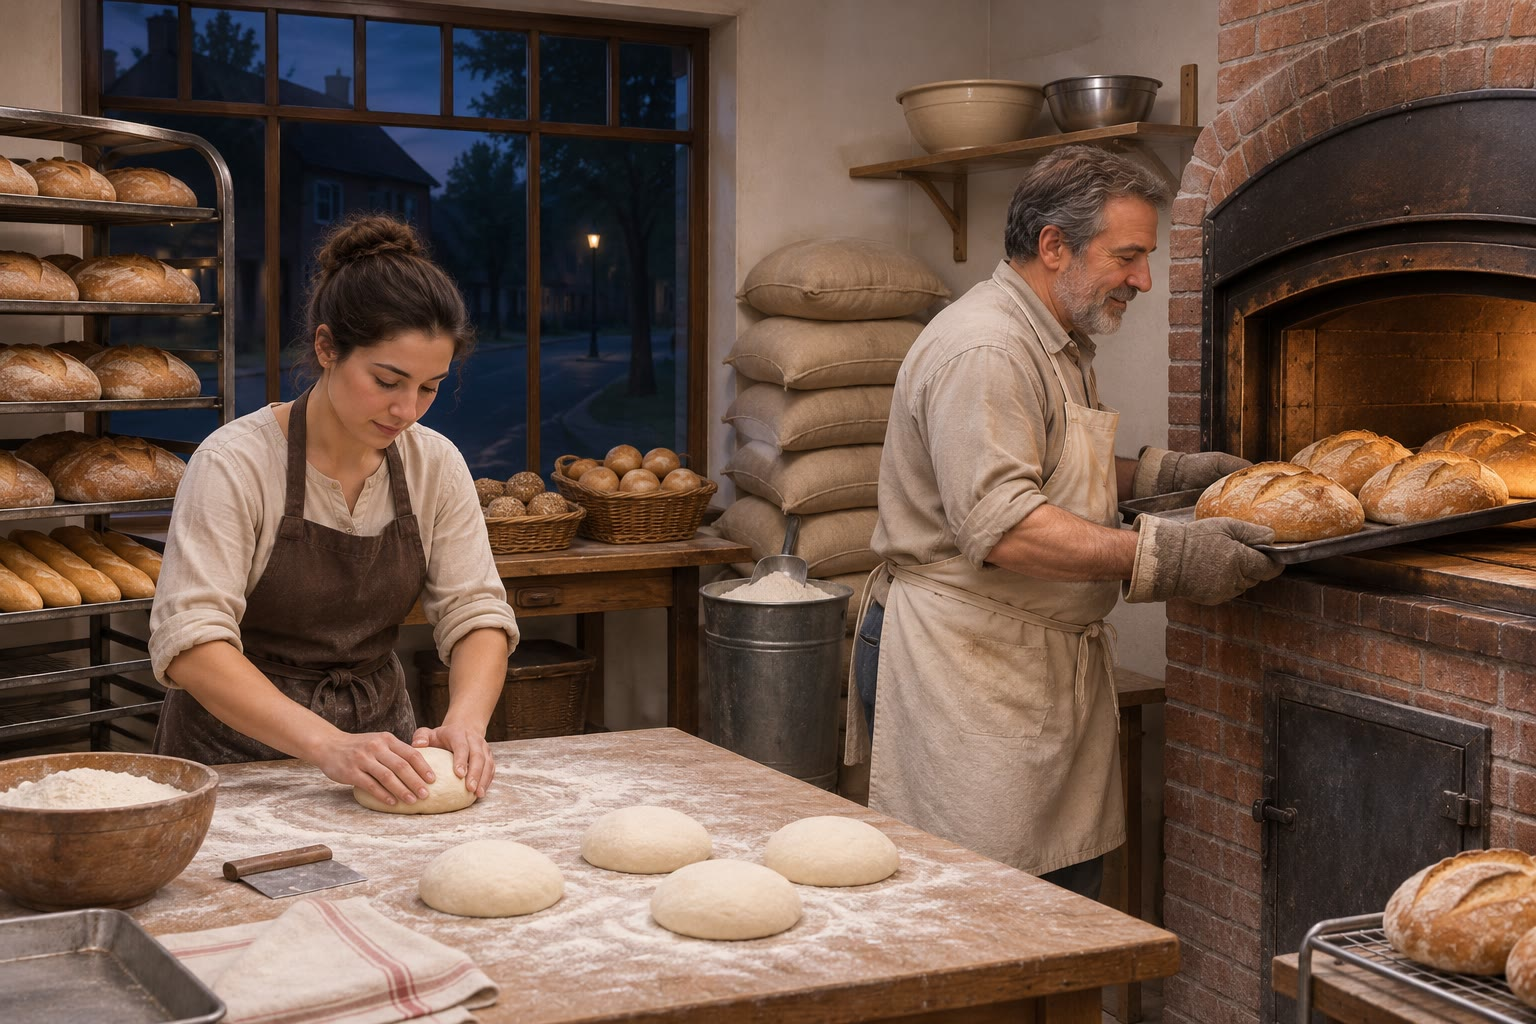
\includegraphics[width=0.52\linewidth]{images/book1/ai/g7-firms-bakery-dawn.jpg}

{\small A bakery before dawn. The oven and the shop cost the same whether one loaf or a
thousand are sold; the flour and the energy grow with each loaf.}
\end{omfigure}

\section{Revenue}

\begin{definition}[Revenue]\label{def:g7:firms:revenue}
The \emph{revenue}\index{revenue} of a \omterm{def:g7:firms:firm}{firm} in a period is the \omterm{def:g7:money:money}{money} it receives from its
sales: for a single good sold at one \omterm{def:g7:money:price}{price},
\[
\text{revenue} = \text{price} \times \text{quantity sold}.
\]
\end{definition}

\begin{example}
A bakery in Brenmoor sells its loaves at 2 dalens each. If it sells $3\,000$ loaves in a month,
its \omterm{def:g7:firms:revenue}{revenue} is $2 \times 3\,000 = 6\,000$ dalens.
\end{example}

\section{Fixed and variable costs}

\begin{definition}[Fixed cost]\label{def:g7:firms:fixed-cost}
A \emph{fixed cost}\index{fixed cost} is a cost that does not depend on the quantity produced
in the period: rent, the hire of machines, insurance.
\end{definition}

\begin{definition}[Variable cost]\label{def:g7:firms:variable-cost}
A \emph{variable cost}\index{variable cost} is a cost that grows with the quantity produced:
materials, energy for each unit, packaging, the pay of workers paid for each unit.
\end{definition}

\begin{definition}[Total cost]\label{def:g7:firms:total-cost}
The \emph{total cost}\index{total cost} of a \omterm{def:g7:firms:firm}{firm} in a period is its \omterm{def:g7:firms:fixed-cost}{fixed cost} plus its
\omterm{def:g7:firms:variable-cost}{variable cost}.
\end{definition}

\begin{example}
The bakery pays $3\,000$ dalens a month for its shop, its oven and its two bakers, whatever it
sells; each loaf costs $0.80$ dalens of flour, yeast, energy and paper bag. For $3\,000$ loaves,
the \omterm{def:g7:firms:variable-cost}{variable cost} is $0.80 \times 3\,000 = 2\,400$ dalens and the \omterm{def:g7:firms:total-cost}{total cost} $3\,000 + 2\,400 =
5\,400$ dalens.
\end{example}

\section{Profit, loss and the break-even quantity}

\begin{definition}[Profit]\label{def:g7:firms:profit}
The \emph{profit}\index{profit} of a \omterm{def:g7:firms:firm}{firm} in a period is its \omterm{def:g7:firms:revenue}{revenue} minus its \omterm{def:g7:firms:total-cost}{total cost}, when
this difference is positive.
\end{definition}

\begin{definition}[Loss]\label{def:g7:firms:loss}
A \omterm{def:g7:firms:firm}{firm} makes a \emph{loss}\index{loss} when its \omterm{def:g7:firms:total-cost}{total cost} is larger than its \omterm{def:g7:firms:revenue}{revenue}; the loss
is the difference.
\end{definition}

% figdata: bakery (q 0 1000 2000 2500 3000 4000; revenue 0 .. 8000; cost 3000 3800 4600 5000 5400 6200;
% profit -3000 -1800 -600 0 600 1800)
For $3\,000$ loaves, the bakery's \omterm{def:g7:firms:profit}{profit} is $6\,000 - 5\,400 = 600$ dalens. The table gives its
\omterm{def:g7:firms:revenue}{revenue}, \omterm{def:g7:firms:total-cost}{total cost} and \omterm{def:g7:firms:profit}{profit} at other quantities in a month.
\begin{center}
\begin{tabular}{lrrrrrr}
\toprule
Loaves sold & 0 & 1\,000 & 2\,000 & 2\,500 & 3\,000 & 4\,000 \\
\midrule
\omterm{def:g7:firms:revenue}{Revenue} (dalens) & 0 & 2\,000 & 4\,000 & 5\,000 & 6\,000 & 8\,000 \\
\omterm{def:g7:firms:total-cost}{Total cost} (dalens) & 3\,000 & 3\,800 & 4\,600 & 5\,000 & 5\,400 & 6\,200 \\
\omterm{def:g7:firms:profit}{Profit} ($+$) or \omterm{def:g7:firms:loss}{loss} ($-$) & $-3\,000$ & $-1\,800$ & $-600$ & 0 & $+600$ & $+1\,800$ \\
\bottomrule
\end{tabular}
\end{center}

\begin{definition}[Break-even quantity]\label{def:g7:firms:break-even}
The \emph{break-even quantity}\index{break-even quantity} is the quantity at which \omterm{def:g7:firms:revenue}{revenue}
equals \omterm{def:g7:firms:total-cost}{total cost}: below it, the \omterm{def:g7:firms:firm}{firm} makes a \omterm{def:g7:firms:loss}{loss}; above it, a \omterm{def:g7:firms:profit}{profit}.
\end{definition}

Each loaf brings in 2 dalens and costs $0.80$ dalens more to make: it leaves $1.20$ dalens to
pay the \omterm{def:g7:firms:fixed-cost}{fixed cost}. To pay $3\,000$ dalens of \omterm{def:g7:firms:fixed-cost}{fixed cost}, the bakery must sell
\[
3\,000 \div 1.20 = 2\,500 \text{ loaves}.
\]
This is its \omterm{def:g7:firms:break-even}{break-even quantity}.

\begin{omfigure}
\begin{tikzpicture}[econ, x=1.5cm, y=0.75cm]
  % x: thousands of loaves; y: thousands of dalens
  \draw[econ axes] (0,8.8) node[above, font=\scriptsize] {thousands of dalens} |- (4.6,0)
    node[right, font=\scriptsize] {loaves};
  \foreach \x/\l in {1/1000, 2/2000, 3/3000, 4/4000}
    \draw (\x,0) -- (\x,-0.12) node[below, font=\scriptsize] {\l};
  \foreach \y in {2,4,6,8} \draw (0,\y) -- (-0.06,\y) node[left, font=\scriptsize] {\y};
  \draw[demand] (0,0) -- (1,2) -- (2,4) -- (2.5,5) -- (3,6) -- (4,8)
    node[right, font=\scriptsize, align=left] {revenue};
  \draw[supply] (0,3) -- (1,3.8) -- (2,4.6) -- (2.5,5) -- (3,5.4) -- (4,6.2)
    node[right, font=\scriptsize] {total cost};
  \draw[guide] (0,3) -- (4,3);
  \node[font=\scriptsize, above] at (3.4,3) {fixed cost};
  \foreach \x/\y in {0/0, 1/2, 2/4, 2.5/5, 3/6, 4/8} \fill[omDef] (\x,\y) circle (1.5pt);
  \foreach \x/\y in {0/3, 1/3.8, 2/4.6, 3/5.4, 4/6.2} \fill[omThm] (\x,\y) circle (1.5pt);
  \draw[guide] (2.5,0) -- (2.5,5);
  \node[eqpoint] at (2.5,5) {};
  \node[font=\scriptsize, above left] at (2.5,5.1) {break-even: 2\,500 loaves};
  \node[font=\scriptsize] at (1.35,3.3) {loss};
  \node[font=\scriptsize] at (3.55,6.5) {profit};
\end{tikzpicture}

{\small The bakery's \omterm{def:g7:firms:revenue}{revenue} and \omterm{def:g7:firms:total-cost}{total cost}, drawn from the table. Left of $2\,500$ loaves the
cost line is above the \omterm{def:g7:firms:revenue}{revenue} line: a \omterm{def:g7:firms:loss}{loss}. Right of it, a \omterm{def:g7:firms:profit}{profit}.}
\end{omfigure}

\begin{measure}[Profit in a firm's accounts]
A \omterm{def:g7:firms:firm}{firm}'s accounts count the costs it pays. They do not count the time of an owner who works
without a \omterm{def:g7:households:wage}{wage}, nor the \omterm{def:g7:money:money}{money} the owner put in, which could have earned interest elsewhere.
These are \omterm{def:g7:scarcity-and-opportunity-cost:opportunity-cost}{opportunity costs}. A bakery that shows a \omterm{def:g7:firms:profit}{profit} of $600$ dalens a month, while its
owner works 50 hours a week in it unpaid, may earn the owner less than a job as a baker would.
Economists subtract these \omterm{def:g7:scarcity-and-opportunity-cost:opportunity-cost}{opportunity costs} before calling a \omterm{def:g7:firms:firm}{firm} profitable.
\end{measure}

\section{Risk, entry and exit}

A \omterm{def:g7:firms:firm}{firm} does not know its sales in advance. A new bakery pays its rent from the first month;
customers come slowly, a competitor may open across the street, the \omterm{def:g7:money:price}{price} of flour may rise.
The \omterm{def:g7:firms:entrepreneur}{entrepreneur} bears the risk: if the \omterm{def:g7:firms:firm}{firm} makes a \omterm{def:g7:firms:loss}{loss}, the owner loses the \omterm{def:g7:money:money}{money} put in.
This is why the possibility of a \omterm{def:g7:firms:profit}{profit} is needed for anyone to open a \omterm{def:g7:firms:firm}{firm}.

\begin{model}{Entry and exit}
\assumes Anyone may open a \omterm{def:g7:firms:firm}{firm} in the \omterm{def:g7:markets-and-prices:market}{market}, or close one; \omterm{def:g7:firms:profit}{profits} and losses can be seen.
\predicts Where \omterm{def:g7:firms:firm}{firms} make high \omterm{def:g7:firms:profit}{profits}, new \omterm{def:g7:firms:firm}{firms} come in; their extra output lowers the \omterm{def:g7:money:price}{price}
towards cost, and \omterm{def:g7:firms:profit}{profits} shrink. Where \omterm{def:g7:firms:firm}{firms} make losses, some close; output falls, the \omterm{def:g7:money:price}{price}
recovers, and the \omterm{def:g7:firms:input}{inputs} they used move to other uses.
\tested Tested in \cref{ch:g8:competition-and-monopoly-first-look}: when new makers of a medicine
enter after its patent ends, its \omterm{def:g7:money:price}{price} falls, the more so the more makers there are. The opening
chart, where many \omterm{def:g7:firms:firm}{firms} are born and close every year, describes entry and exit; it does not test
whether \omterm{def:g7:firms:profit}{profits} draw entry.
\breaks When a licence, a patent or a very large \omterm{def:g7:firms:fixed-cost}{fixed cost} keeps new \omterm{def:g7:firms:firm}{firms} out, high \omterm{def:g7:firms:profit}{profits} can
last (\cref{ch:g8:competition-and-monopoly-first-look}).
\end{model}

\begin{omchart}{Of 100 firms born in 2021 in the European Union, how many were still active
three years later, by sector.}{Eurostat, business demography (bd\_size), three-year survival
rate of enterprises newly born in 2021, European Union}
\begin{tikzpicture}
\begin{axis}[omrecord, xbar, bar width=7pt, xmin=0, xmax=80, ytick=data,
  yticklabels from table={figdata/grade-7/08-firms/out/survival_sector.csv}{label},
  y tick label style={font=\scriptsize}, xlabel={Firms still active after three years (of 100)},
  height=0.48\linewidth, width=0.6\linewidth, enlarge y limits=0.06,
  nodes near coords, nodes near coords align={horizontal}, every node near coord/.append style={font=\scriptsize}]
\addplot[fill=omDef, draw=none] table[x=value, y=pos] {figdata/grade-7/08-firms/out/survival_sector.csv};
\end{axis}
\end{tikzpicture}
\end{omchart}

% figdata: survival_sector (transport 43.8 ... health 67.5); brenland_sectors (services 326 firms, 69 with a loss,
% 21.2 %; manufacturing 123, 1, 0.8 %; farming 51, 0; margin 31.8, 26.8, 13.5)
The risk is not the same everywhere. Of 100 \omterm{def:g7:firms:firm}{firms} born in transport and storage, $43.8$ were
still active after three years; in health and social work, $67.5$. A closure is not always a
failure: some owners retire, sell their \omterm{def:g7:firms:firm}{firm}, or merge it with another. The survival rates do not
say why a \omterm{def:g7:firms:firm}{firm} closed.

In Brenland's census of 500 \omterm{def:g7:firms:firm}{firms} (invented), $69$ of the $326$ service \omterm{def:g7:firms:firm}{firms} made a \omterm{def:g7:firms:loss}{loss} in
2025, that is $21.2\,\%$, against $1$ of $123$ manufacturing \omterm{def:g7:firms:firm}{firms} and none of the 51 farms.

\section{Exercises}

\begin{exercise}[$\star$]\label{exo:g7:firms:1}
Use the opening chart. Of 100 \omterm{def:g7:firms:firm}{firms} born in the European Union in 2021, how many were still
active after three years? How many had closed?
\end{exercise}

\begin{exercise}[$\star$]\label{exo:g7:firms:2}
A sandwich shop sells 350 sandwiches at $4.50$ dalens each in a week. What is its \omterm{def:g7:firms:revenue}{revenue}?
\end{exercise}

\begin{exercise}[$\star$]\label{exo:g7:firms:3}
A workshop has a \omterm{def:g7:firms:fixed-cost}{fixed cost} of $1\,200$ dalens a week and a \omterm{def:g7:firms:variable-cost}{variable cost} of $2.10$ dalens per
unit. What is its \omterm{def:g7:firms:total-cost}{total cost} for 300 units?
\end{exercise}

\begin{exercise}[$\star$]\label{exo:g7:firms:4}
A \omterm{def:g7:firms:firm}{firm} has a \omterm{def:g7:firms:revenue}{revenue} of $1\,575$ dalens and a \omterm{def:g7:firms:total-cost}{total cost} of $1\,830$ dalens in a week. Does it
make a \omterm{def:g7:firms:profit}{profit} or a \omterm{def:g7:firms:loss}{loss}, and of how much?
\end{exercise}

\begin{exercise}[$\star\star$]\label{exo:g7:firms:5}
A \omterm{def:g7:firms:firm}{firm} sells at 5 dalens a unit, with a \omterm{def:g7:firms:fixed-cost}{fixed cost} of 800 dalens and a \omterm{def:g7:firms:variable-cost}{variable cost} of 3 dalens
per unit. Make a table of \omterm{def:g7:firms:revenue}{revenue}, \omterm{def:g7:firms:total-cost}{total cost} and \omterm{def:g7:firms:profit}{profit} for 200, 300, 400 and 500 units. What is
the \omterm{def:g7:firms:break-even}{break-even quantity}?
\end{exercise}

\begin{exercise}[$\star\star$]\label{exo:g7:firms:6}
A \omterm{def:g7:firms:firm}{firm} has a \omterm{def:g7:firms:fixed-cost}{fixed cost} of $2\,400$ dalens, sells at 6 dalens a unit and has a \omterm{def:g7:firms:variable-cost}{variable cost} of 2
dalens per unit. Compute its \omterm{def:g7:firms:break-even}{break-even quantity}.
\end{exercise}

\begin{exercise}[$\star\star$]\label{exo:g7:firms:7}
The rent of the chapter's bakery rises, and its \omterm{def:g7:firms:fixed-cost}{fixed cost} goes from $3\,000$ to $3\,600$ dalens a
month. \omterm{def:g7:money:price}{Price} and \omterm{def:g7:firms:variable-cost}{variable cost} do not change. What is the new \omterm{def:g7:firms:break-even}{break-even quantity}? By how many
loaves did it rise?
\end{exercise}

\begin{exercise}[$\star\star$]\label{exo:g7:firms:8}
Use the Brenland census. Which sector has the largest share of \omterm{def:g7:firms:firm}{firms} making a \omterm{def:g7:firms:loss}{loss}? Compute the
share of all 500 \omterm{def:g7:firms:firm}{firms} that made a \omterm{def:g7:firms:loss}{loss}, in percent.
\end{exercise}

\begin{exercise}[$\star\star$]\label{exo:g7:firms:9}
Describe an observation that would contradict the model ``Entry and exit''.
\end{exercise}

\begin{exercise}[$\star\star\star$]\label{exo:g7:firms:10}
The chapter's bakery cuts its \omterm{def:g7:money:price}{price} from 2 dalens to $1.80$ dalens. (a) How much does each loaf
now leave to pay the \omterm{def:g7:firms:fixed-cost}{fixed cost}? (b) What is the new \omterm{def:g7:firms:break-even}{break-even quantity}? (c) At $3\,000$ loaves,
what is the new \omterm{def:g7:firms:profit}{profit}?
\end{exercise}

\begin{exercise}[$\star\star\star$]\label{exo:g7:firms:11}
Bakeries in a town make high \omterm{def:g7:firms:profit}{profits}, and many new bakeries open. Predict, with the model ``Entry
and exit'', what happens to the \omterm{def:g7:money:price}{price} of bread, to the \omterm{def:g7:firms:profit}{profit} of each bakery, and to the number of
bakeries after a few years.
\end{exercise}

\begin{exercise}[$\star\star\star$]\label{exo:g7:firms:12}
The opening chart shows how many \omterm{def:g7:firms:firm}{firms} are still active. Name two questions about why \omterm{def:g7:firms:firm}{firms} close
that it cannot answer.
\end{exercise}

\section{Problem: Opening a Juice Stall}

\begin{problem}[{Weekend problem --- the costs of a juice stall, revenue and profit at three
prices, and a second stall next door}]
\label{pb:g7:firms:1}
Everything in this problem is invented. Mira opens a juice stall at the Brenmoor \omterm{def:g7:markets-and-prices:market}{market}. The
stall and its blender cost 600 dalens a month, whatever she sells. Each cup needs $0.90$ dalens of
fruit and a cup that costs $0.10$ dalens.

\medskip
\noindent\textbf{Part I --- Costs.}
\begin{enumerate}
  \item What is Mira's \omterm{def:g7:firms:fixed-cost}{fixed cost} per month? Her \omterm{def:g7:firms:variable-cost}{variable cost} per cup?
  \item What is her \omterm{def:g7:firms:total-cost}{total cost} for 500 cups in a month?
  \item Which cost must she pay even in a month when she sells nothing?
  \item At 500 cups, what is the \omterm{def:g7:firms:total-cost}{total cost} per cup?
\end{enumerate}

\medskip
\noindent\textbf{Part II --- Revenue and profit.} Mira tries three \omterm{def:g7:money:price}{prices} in three months. She
sells 600 cups at $2.50$ dalens, 500 cups at 3 dalens, and 250 cups at 4 dalens.
\begin{enumerate}[resume]
  \item Compute her \omterm{def:g7:firms:revenue}{revenue} at each \omterm{def:g7:money:price}{price}.
  \item Compute her \omterm{def:g7:firms:total-cost}{total cost} in each month.
  \item Compute her \omterm{def:g7:firms:profit}{profit} in each month. Which \omterm{def:g7:money:price}{price} gave the largest \omterm{def:g7:firms:profit}{profit}?
  \item At 3 dalens a cup, what is her \omterm{def:g7:firms:break-even}{break-even quantity}?
\end{enumerate}

\medskip
\noindent\textbf{Part III --- A second stall.} A second juice stall opens next door. At 3
dalens, Mira now sells only 280 cups a month; at $2.50$ dalens, 420 cups.
\begin{enumerate}[resume]
  \item What is Mira's \omterm{def:g7:firms:profit}{profit} or \omterm{def:g7:firms:loss}{loss} at 3 dalens?
  \item What is her \omterm{def:g7:firms:profit}{profit} or \omterm{def:g7:firms:loss}{loss} at $2.50$ dalens?
  \item What is her \omterm{def:g7:firms:break-even}{break-even quantity} at $2.50$ dalens?
  \item What does the model ``Entry and exit'' predict if a third stall opens? Use your answers.
\end{enumerate}
\end{problem}
